\documentclass{book}
\usepackage{../sty/latexmldoc}
\usepackage{makeidx}
\input{release.tex}
\makeindex

\title{\LaTeXML\ \emph{The Manual}}
\subtitle{A \LaTeX\ to \XML\ Converter;\\ \emph{\CurrentVersion}}
\author{Bruce R.~Miller}
\begin{document}
\frontmatter
\maketitle
\tableofcontents
\mainmatter
%%%======================================================================
\chapter{Introduction}\label{intro}
For many, \LaTeX\ is the prefered format for document authoring, particularly those
involving significant mathematical content and where quality typesetting is desired.
On the other hand, content-oriented \XML\ is an extremely useful representation for documents,
allowing them to be used, and reused, for a variety of purposes, not least, 
presentation on the Web. Yet, the style and intent of \LaTeX\ markup, as compared to \XML\
markup, not to mention its programmability, presents difficulties in converting
documents from the former format to the latter.
Perhaps ironically, these difficulties can be particularly large for mathematical material, 
where there is a tendency for the markup to focus on appearance rather than meaning.

The choice of \LaTeX\ for authoring, and \XML\ for delivery were natural and uncontroversial
choices for the \URL[Digital Library of Mathematical Functions]{http://dlmf.nist.gov}.
Faced with the need to perform this conversion and the lack of suitable tools to perform it, 
the DLMF project proceeded to develop thier own tool, \LaTeXML, for this purpose.
This document describes a \emph{preview} release of \LaTeXML.

\paragraph{Design Goals} The idealistic goals of \LaTeXML\ are:
\begin{itemize}
\item Faithful emulation of \TeX's behaviour.
\item Easily extensible.
\item Lossless; preserving both semantic and presentation cues.
\item Uses abstract \LaTeX-like, extensible, document type.
\item Determine the semantics of mathematical content\\
    (\emph{Good} Presentation \MathML, eventually Content \MathML\ and \OpenMath).
\end{itemize}

As these goals are not entirely practical, or even somewhat contradictory,
they are implicitly modified by ``as much as possible.''
Completely mimicing \TeX's behaviour would seem to require the sneakiest modifications
to \TeX, itself.  `Ease of use' is, of course, in the eye of the beholder.
More significantly, few documents are likely to have completely unambiguous
mathematics markup; human understanding of both the topic and the surrounding 
text is needed to properly interpret any particular fragment.
Thus, rather than pretend to provide a `turn-key' solution,
we expect that document-specific declarations or tuning to be necessary
to faithfully convert documents.  Towards this end, we provide a variety
of means to customize the processing and declare the author's intent.
At the same time, especially for new documents, we encourage a more logical, 
content-oriented markup style, over a purely presentation-oriented style.

\paragraph[Overview]{Overview of this Manual}
Chapter \ref{usage} describes the usage of \LaTeXML, along with
common use cases and techniques.  Chapter \ref{architecture} describes
the system architecture in some detail. Strategies for customization
and implementation of new packages is described in Chapter \ref{customization}.
The special considerations for mathematics, including details of representation
and how to improve the conversion, are covered in Chapter \ref{math}.
An overview of outstanding issues and planned future improvements
are given in Chapter \ref{todo}.
Finally, the Appendices \ref{commands}, \ref{coremodules} give detailed documentation
on the commands and modules comprising the system.

If all else fails, you can consult the source code, or the author.

%%%======================================================================
\chapter{Using \LaTeXML}\label{usage}
The main commands provided by the \LaTeXML\ system are
\begin{description}
\item[\ltxcmd{latexml}] for converting \TeX\ sources to \XML.
\item[\ltxcmd{latexmlpost}] for various postprocessing tasks including
conversion to \HTML, processing images, conversion to \MathML\ and so on.
\end{description}
The usage of these commands can be as simple as
\begin{quote}
 \cmd{latexml doc.tex | latexmpost --dest=doc.xhtml}
\end{quote}
to convert a single document into \HTML,  or as complicated as
\begin{quote}
 \cmd{latexml --dest=A.xml doca}\\
 \cmd{latexml --dest=B.xml docb}\\
  \hbox{}\hspace{1in}\ldots\\
 \cmd{latexmlpost --prescan --dbfile=my.db --dest=A.xhtml A}\\
 \cmd{latexmlpost --prescan --dbfile=my.db --dest=B.xhtml B}\\
  \hbox{}\hspace{1in}\ldots\\
 \cmd{latexmlpost --noscan --dbfile=my.db --dest=A.xhtml A}\\
 \cmd{latexmlpost --noscan --dbfile=my.db --dest=B.xhtml B}\\
  \hbox{}\hspace{1in}\ldots
\end{quote}
to convert a whole set of documents into a complete site.

How best to use the commands depends, of course, on what you
are trying to achieve.  In the next section, we'll describe
the use of \ltxcmd{latexml}, which will be sufficient
if the \XML\ representation is what you want, or if you
intend to carry out any further processing with your own
\XML-tools.  The following sections consider a sequence of
successively more complicated postprocessing situations,
using \ltxcmd{latexmlpost},
in which one or more \TeX\ sources can be converted into
one or more web documents or a complete site.

%%%----------------------------------------------------------------------
\section[Conversion]{Basic \XML\ Conversion}\label{usage.conversion}\index{latexml!usage}
The command
\begin{quote}
 \cmd{latexml \textit{options} --destination=\varfile[xml]{doc} \varfile{doc}}
\end{quote}
loads any required definition modules (see below),
reads, tokenizes, expands and digests the \TeX\ document \texttt{doc.tex}
(or from standard input, if \texttt{-} is given for the filename),
converts it to \XML,
performs some document rewriting, parses the mathematical content
and writes the result in \texttt{doc.xml}.
For details on the processing, see Chapter \ref{architecture},
and Chapter \ref{math} for more information about math parsing.

\paragraph{Module Loading}
A first consideration is what definitions for control sequences and
environments are active and used for the processing.
Definitions and customization modules, if present, are loaded in the following
order:
\begin{description}
  \item[\texttt{TeX.pool.ltxml}] the core module is always loaded.
  \item[\cmd{--preload=\varfile{module}}] causes loading of \varfile[ltxml]{module}.
    For example, if \LaTeXML\ fails to recognize a \LaTeX\ document 
    \cmd{--preload=LaTeX.pool} can be useful to force \LaTeX-mode.
    Or if you want
    This option can be repeated, and the modules will be loaded in the
    given order.
  \item[\varfile{doc}\texttt{.latexml}] a document-specific customization module
    is loaded if present.
\end{description}
As processing proceeds, additional modules may be loaded as follows.
\begin{description}
  \item[\texttt{LaTeX.pool.ltxml}] the core latex module, is loaded
    upon encountering certain recognizably \LaTeX-specific commands, such as
    \verb|\documentclass|.
  \item[\code{\cs{documentclass}\{\varfile{class}\}}]
     loads \varfile[cls.ltxml]{class}.
     (legacy \verb|\documentstyle| behaves similarly, along with any required packages).
  \item[\code{\cs{usepackage}\{\textit{package}\}}] (or related) loads
    \varfile[sty.ltxml]{package}.  \LaTeXML\ will not
    attempt to read the \varfile[sty]{package} file, as these
    often involve \LaTeX\ internals meaningless to the generation of \XML,
    unless forced to with the option
    \begin{quote}
      \cmd{--includestyles}
    \end{quote}
    A selective, per-file, option may be developed in the future --- please
    provide use cases.
  \item[\code{\cs{input}\{\varfile{file}\}}] loads an appropriate version
     of \varfile{file}, specifically the first found of:
    \varfile[tex.ltxml]{file}, \varfile[tex]{file}, 
    \varfile[ltxml]{file} or \varfile{file}.
\end{description}
Some of these modules (esp.~\code{TeX} and \code{LaTeX}), are parts of
the \LaTeXML\ distribution; others are supplied by the user, or can be
overridden by the user.
See Chapter \ref{customization} for details about what can go in these modules.

Directories to search (in addition to the working directory)
for modules and other files can be specified using
\begin{quote}
  \cmd{--path=\varfile{directory}}
\end{quote}
This option can be repeated.

\paragraph{Other Options}
The number and detail of progress and debugging messages printed
during processing can be controlled using
\begin{quote}
  \cmd{--verbose} and \cmd{--quiet}
\end{quote}
They can  be repeated to get even more or fewer details.

An option most useful in constructing complicated sites is
\begin{quote}
  \cmd{--documentid=\textit{id}}
\end{quote}
which provides an ID for the document root element which is inheritted
as a prefix for id's of the child-elements in the document.
Using this option can assure unique identifiers across a set
of source documents.

See the documentation for the command \ltxcmd{latexml} for
less common options.

%%%----------------------------------------------------------------------
\section[Postprocessing]{Basic Postprocessing}\label{usage.single}\index{latexmlpost!usage}
In the simplest situation, you have a single \TeX\ source document
from which you want to generate a single output document.
The command
\begin{quote}
 \cmd{latexmlpost \textit{options} --destination=doc.xhtml doc}
\end{quote}
or similarly with \code{--destination=doc.html},
will carry out a set of appropriate transformations in sequence:
\begin{itemize}
  \item scanning of labels and ids;
  \item filling in the index and bibliography (if needed);
  \item cross-referencing;
  \item conversion of math;
  \item conversion of graphics and picture environments to web format (png);
  \item applying an \XSLT\ stylesheet.
\end{itemize}
The output format affects the defaults for each step and is determined
by the file extension of \code{--destination}, or by the option
\begin{quote}
 \cmd{--format=(xhtml|html|xml)}
\end{quote}
\begin{description}
 \item[html] both math and graphics are converted to png images;
    the stylesheet \code{LaTeXML-html.xslt} is used.
 \item[xhtml] math is converted to Presentation \MathML, other graphics are converted to images;
    the stylesheet \code{LaTeXML-xhtml.xslt}  is used.
 \item[xml] no math, graphics or \XSLT\ conversion is carried out.
\end{description}
Of course, all of these conversions can be controlled or overridden
by explicit options described below.
For more details about less common options, see the command
documentation \ltxcmd{latexmlpost}, as well as Appendix \ref{postmodules}.

\paragraph{Scanning}
The scanning step collects information about all labels, ids,
indexing commands, cross-references and so on, to be used
in the following postprocessing stages.

\paragraph{Indexing}
An index is built from \verb|\index| markup, if
\code{makeidx}'s \verb|\printindex| command has been used,
but this can be disabled by
\begin{quote}
  \cmd{--noindex}
\end{quote}
The index entries can be permuted with the option
\begin{quote}
  \cmd{--permutedindex}
\end{quote}
Thus \verb|\index{term a!term b}| also shows up as \verb|\index{term b!term a}|.
This leads to a more complete, but possibly rather silly, index,
depending on how the terms have been written.

\paragraph{Bibliography}
Bibilographic data from BibTeX can be provided with the option
\begin{quote}
  \cmd{--bibliography=\varfile[xml]{bibfile}}
\end{quote}
However, the tools to convert a BibTeX file to \XML\ are
not yet provided with the distribution.

\paragraph{Cross-Referencing}
In this stage, the scanned information is used to fill in the
text and links of cross-references within the document.
The option
\begin{quote}
  \cmd{--urlstyle=(server|negotiated|file)}
\end{quote}
can control the format of urls with the document.
\begin{description}
  \item[server] formats urls appropriate for use from a web server.
    In particular, trailing \code{index.html} are omitted. (default)
  \item[negotiated] formats urls appropriate for use by a server
    that implements content negotiation. File extensions for \code{html}
    and \code{xhtml} are omitted.  This enables you to set up a server
    that serves the appropriate format depending on the browser being used.
  \item[file] formats urls explicitly, with full filename and extension.
    This allows the files to be browsed from the local filesystem.
\end{description}

\paragraph{Math Conversion}
Specific conversions of the mathematics can be requested
using the options
\begin{quote}
 \code{--mathimages}   converts math to png images,\\
 \code{--presentationmathml} (or \code{--pmml}) creates Presentation \MathML\\
 \code{--contentmathml} (or \code{--cmml}) creates Content \MathML\\
 \code{--openmath} (or \code{--om}) creates \OpenMath
\end{quote}
(Each of these options can also be negated if needed, eg.~\code{--nomathimages})
It must be pointed out that the Content \MathML\ and \OpenMath\
conversions are currently rather experimental.

More than one of these conversions can be requested, and
each will be included in the output document.
However, the option
\begin{quote}
 \code{--parallelmath}
\end{quote}
can be used to generate parallel \MathML\ markup, provided the first
conversion is either \code{--pmml} or \code{--cmml}.

\paragraph[Graphics]{Graphics processing}
Conversion of graphics (eg.~from the \code{graphic(s|x)} packages' 
\verb|\includegraphics|) can be enabled or disabled
using
\begin{quote}
 \code{--graphicsimages} or \code{--nographicsimages}
\end{quote}
Similarly, the conversion of \code{picture} environments can be controlled with
\begin{quote}
 \code{--pictureimages} or \code{--nopictureimages}
\end{quote}
An experimental capability for converting the latter to \textsc{SVG} can be
controlled by
\begin{quote}
 \code{--svg} or \code{--nosvg}
\end{quote}

\paragraph{Stylesheet}
If you wish to provide your own \XSLT\  or
\CSS\ stylesheets, the options 
\begin{quote}
\code{--stylesheet=\varfile[xsl]{stylesheet}}\\
\code{--css=\varfile[css]{stylesheet}}
\end{quote}
 can be used.  The \code{--css} option can be repeated to include multiple stylesheets;
for example, the distribution provides several in addition to the \code{core.css} stylesheet
which is included by default.
\begin{description}
\item[\code{navbar-left.css}] Places a navigation bar on the left.
\item[\code{navbar-right.css}] Places a navigation bar on the left.
\item[\code{theme-blue.css}] Colors various features in a soft blue.
\item[\code{amsart.css}] A style appropriate for many journal articles.
\end{description}

To develop such stylesheets, a knowledge
of the \LaTeXML\ document type is necessary; See Appendix \ref{schema}.

%%%----------------------------------------------------------------------
\section[Splitting]{Splitting the Output}\label{usage.multiple}\index{latexmlpost!usage!split pages}
For larger documents, it is often desirable to break the 
result into several interlinked pages. This split,
carried out before scanning, is requested by 
\begin{quote}
 \cmd{--splitat=\textit{level}}
\end{quote}
where \textit{level} is one of \texttt{chapter},
\texttt{section}, \texttt{subsection}, or \texttt{subsubsection}.
For example, \texttt{section} would split the document into
chapters (if any) and sections, along with separate
bibliography, index and any appendices.
The removed document nodes are replaced by a Table of Contents.

The extra files are named using either the id or label
of the root node of each new page document according to
\begin{quote}
  \cmd{--splitnaming=(id|idrelative|label|labelrelative)}
\end{quote}
The relative foms create shorter names in subdirectories for each
level of splitting.
The \code{--urlstyle} option may also be useful here,
as well as the \ltxcmd{latexml} option \code{--documentid}.

Additionally, the index and bibliography can be split
into separate pages according to the initial letter of entries by using the options
\begin{quote}
  \cmd{--splitindex} and \cmd{--splitbibliography}
\end{quote}

%%%----------------------------------------------------------------------
\section[Sites]{Site processing}\label{usage.site}\index{latexmlpost!usage!site}
A more complicated situation combines several \TeX\ sources
into a single interlinked site consisting of multiple pages
and a composite index and bibliography.
The games one must play with \LaTeX's aux files to satisfy cross-references
between these documents are not covered here, but the situation is handled
by \LaTeXML\ in the following fashion.

\begin{description}
\item[Conversion] First, all \TeX\ sources must be converted
   to \XML, using \ltxcmd{latexml}.  Since every target-able element
   in all files to be combined must have a unique identifier, it is useful to
   prefix each identifier with a unique value for each file. 
   The \ltxcmd{latexml} option \code{--documentid=\textit{id}} provides this.

 \item[Scanning] Secondly, all \XML\ files must be split and scanned using
  the command
  \begin{quote}
   \cmd{latexmlpost --prescan --dbfile=\varfile{DB} --dest=\varfile[xhtml]{i} \varfile{i}}
  \end{quote}
  where \varfile{DB} names a file in which to store the scanned data.
  Other conversions, including writing the output file, are skipped in this prescanning step.
 
 \item[Pagination] Finally, all \XML\ files are cross-referenced and converted into
   the final format using the command
   \begin{quote}
     \cmd{latexmlpost --noscan --dbfile=\varfile{DB} --dest=\varfile[xhtml]{i} \varfile{i}}
   \end{quote}
   which skips the unnecessary scanning step.
\end{description}

%%%======================================================================
\chapter{Architecture}\label{architecture}
Like \TeX, \LaTeXML\ is data-driven: the text and executable control
sequences (ie.~macros and primitives)
in the source file (and any packages loaded) direct the processing.
The user exerts control over the conversion, and customizes it, by 
providing alternative \LaTeXML-specific implementations of the control sequences and packages,
by declaring properties of the desired document structure,
and by defining rewrite rules to be applied to the constructed document tree.

\begin{figure}[tb]
\begin{center}
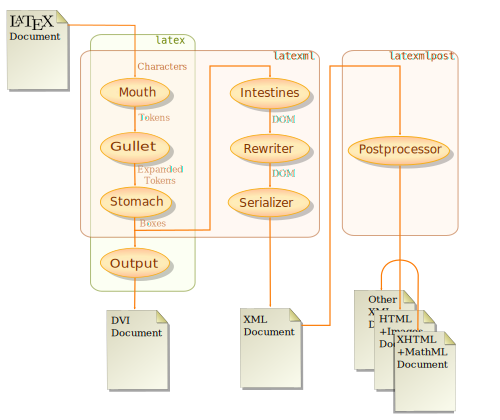
\includegraphics{figures/digestion}
\end{center}
\caption{Flow of data through \LaTeXML's digestive tract.\label{fig:dataflow}}
\end{figure}
The top-level class, \pod{LaTeXML}, manages the processing, providing several methods
for converting a \TeX\ document or string into an \XML\ document, with varying degrees
of postprocessing and optionally writing the document to file.
A \pod{LaTeXML::State} object maintains the current state
of processing, current definitions for control sequences and emulates the
\TeX's scoping rules.
The processing is broken into the following stages
\begin{description}
 \item[Digestion] the \TeX-like digestion phase which converts the input into boxes.
 \item[Construction] converts the resulting boxes into an \XML\ DOM.
 \item[Rewriting] applies rewrite rules to modify the DOM.
 \item[Math Parsing] parses the tokenized mathematics.
\end{description}
See Figure \ref{fig:dataflow} for illustration.
The first three stages are discussed in the following sections;
the parsing of mathematics is covered in detail in Chapter \ref{math}.

The \pod{LaTeXML} object binds \verb|$STATE|, \verb|$GULLET|, \verb|$STOMACH|,
and \verb|$MODEL| to corresponding active objects during processing.

%%%----------------------------------------------------------------------
\section{Digestion}\label{architecture.digestion}
Digestion is carried out primarily in a \emph{pull} mode: The \pod{LaTeXML::Stomach}
pulls expanded \pod{LaTeXML::Token}s from the \pod{LaTeXML::Gullet}, which itself pulls tokens from 
the \pod{LaTeXML::Mouth}.  The \pod{LaTeXML::Mouth} converts characters from the plain text input
into tokens according to the current category codes assigned to them (in the \pod{LaTeXML::State}).  
The \pod{LaTeXML::Gullet} is responsible for expanding any macro or expandible
tokens (when the current binding of the token in the \pod{LaTeXML::State} is 
an \pod{LaTeXML::Expandable} definition), 
and for parsing sequences of tokens into common core datatypes (numbers, dimensions, etc.).
The \pod{LaTeXML::Stomach} digests these tokens by executing \pod{LaTeXML::Primitive} control 
sequences (generally for side effect), converting control sequences bound
to \pod{LaTeXML::Constructor}s into \pod{LaTeXML::Whatsit}s, and converting the remaining tokens
into a recursive structure consisting of
\pod{LaTeXML::Box}es and \pod{LaTeXML::List}s and of \pod{LaTeXML::Box}es.

%%%----------------------------------------------------------------------
\section{Construction}\label{architecture.construction}
The main (intentional) deviation of \LaTeXML's digestion from that of \TeX\ is in the
extension of control sequences to include \pod{LaTeXML::Constructor}s responsible for constructing
\XML\ document fragments, and \pod{LaTeXML::Whatsit}s to represent thier digested form including
whatever arguments were passed to the control sequence.

\emph{Construction} thus consists of creating an \pod{LaTeXML::Document}, containing
an \pod{XML::LibXML::Document} structure, and having it absorb the digested lists, boxes
and whatsits.  Generally, boxes represent text which is converted to text nodes within the
document. Whatsits generally create a document fragment involving elements, attributes
and text.  

A \pod{LaTeXML::Model} is maintained througout the digestion phase which accumulates
any document model declarations in particular the document type (currently only
the DTD, but eventually may be RelaxNG based).  As \LaTeX\ markup is more
like \SGML\ than \XML, declarations may be used to indicate which elements may
be automatically opened or closed when needed to build a document tree that matches
the document type.  As an example, a \verb|<subsection>| will automaticall be closed
when a \verb|<section>| is begun.

%%%----------------------------------------------------------------------
\section{Rewriting}\label{architecture.rewriting}
Once the basic document is constructed, \pod{LaTeXML::Rewrite} rules are applied which can
perform various functions. Ligatures and combining mathematics digits and letters (in certain fonts)
into composite math tokens are handled this way.  Additionally, declarations
of the type or grammatical role of math tokens can be applied here.


%%%======================================================================
\chapter{Customization}\label{customization}
The processsing of the \LaTeX\ document and its  conversion into \XML\ is affected
by the definitions of control sequences, either as macros, primitives or constructors, 
and other declarations specifying the document type, properties of \XML\ tags, ligatures, \ldots.
These definitions and declarations are typically contained in `packages' which provide
the implementation of \LaTeX\ classes and packages.  For example, the \LaTeX\ directive
\verb|\usepackage{foo}| would cause \LaTeXML\ to load the file \code{foo.sty.ltxml}.
This file would be sought in any of the directories in perl's \verb|@INC| list (typically
including the current directory), or in a \verb|LaTeXML/Package| subdirectory of any of 
those directories.  If no such file is found, \LaTeXML\ would look for \code{foo.sty} and
attempt to process it.

When processing a typical file, say \varfile[tex]{jobname}, 
the following packages are loaded:
\begin{enumerate}
\item the core \code{TeX} package
\item any packages named with the \verb|--preload| option,
\item a file \varfile[latexml]{jobname}, if present;
      this provides for document-specific declarations.
\end{enumerate}
Document processing then commences; by default, \LaTeXML\ assumes that the document is plain \TeX.
However, if a \verb|\documentclass| directive is encountered, the \code{LaTeX} package, as well
as a package for the named document class are loaded.

\LaTeXML\ implementations are provided for a number of the standard \LaTeX\ packages,
although many implement only part of the functionality.  Contributed implementations are,
of course, welcome.  These files, as well as the document specific \varfile[latexml]{jobname},
are essentially Perl modules, but use the facilities described in \pod{LaTeXML::Package}.

Much more needs to be explained here, but for the time being,
please consult the documentation for the module \pod{LaTeXML::Package}, and
the various implementations of packages included with the distribution.

%%%======================================================================
\chapter{Mathematics}\label{math}
There are several issues that have to be dealt with in treating the mathematics.
On the one hand, the \TeX\ markup gives a pretty good indication of what the
author wants the math to look like, and so we would seem to have a good handle
on the conversion to presentation forms.  On the other hand, content formats
are desirable as well; there are a few, but too few, clues about what the
intent of the mathematics is.  And in fact, the generation of even Presentation
MathML of high quality requires recognizing the mathematical structure, if not
the actual semantics. The mathematics processing must therefore preserve the
presentational information provided by the author, while inferring, likely
with some help, the mathematical content.

From a parsing point of view, the \TeX-like processing serves as the lexer,
tokenizing the input which \LaTeXML\ will then parse
[perhaps eventually a type-analysis phase will be added].
Of course, there are a few twists.
For one, the tokens, represented by \elementref{XMTok}, can carry extra attributes
such as font and style, but also the name, meaning and grammatical role,
with defaults that can be overridden by the author --- more on those, in a moment.
Another twist is that, although \LaTeX's math markup is not nearly
as semantic as we might like, there is considerable semantics and structure in the 
markup that we can exploit. For example, given a \verb|\frac|, we've already
established the numerator and denominator which can be parsed individually,
but the fraction as a whole can be directly represented as an application,
using \elementref{XMApp}, of a fraction operator; the resulting structure can be treated
as atomic within its containing expression.This \emph{structure preserving} character
greatly simplifies the parsing task and helps reduce misinterpretation.

The parser, invoked by the postprocessor, works only with the top-level lists of lexical tokens,
or with those sublists contained in an \elementref{XMArg}.  The grammar works primarily through
the name and grammatical role.  The name is given by an attribute, or the content if it is
the same.  The role (things like ID, FUNCTION, OPERATOR, OPEN, \ldots) is also given
by an attribute, or, if not present, the name is looked up in a document-specific
dictionary (\varfile[dict]{jobname}), or in a default dictionary.

Additional exceptions that need fuller explanation are: 
\begin{itemize}
 \item \pod{LaTeXML::Constructor}s may wish to create a dual object (\elementref{XMDual}) whose children are 
the semantic and presentational forms.
 \item Spacing and similar markup generates \elementref{XMHint} elements, which are currently ignored
during parsing, but probably shouldn't.
\end{itemize}

%%%----------------------------------------------------------------------
\section{Math Details}\label{math.details}
\LaTeXML\ processes mathematical material by proceeding through several stages:
\begin{itemize}
\item Basic processing of macros, primitives and constructors resulting in
   an XML document; the math is primarily represented by a sequence of
   tokens (\elementref{XMTok}) or structured items (\elementref{XMApp}, \elementref{XMDual}) and
   hints (\elementref{XMHint}, which are ignored).
\item Document tree rewriting, where rules are applied to modify the document tree.
   User supplied rules can be used here to clarify the intent of markup used in the document.
\item Math Parsing; a grammar based parser is applied, depth first, to each level of the math.
   In particular, at the top level of each math expression, as well as each
   subexpression within structured items (these will have been contained in
   an \elementref{XMArg} or \elementref{XMWrap} element).  This results in an expression tree
   that will hopefully be an accurate representation of the expression's structure,
   but may be ambigous in specifics (eg.`what the meaning of a superscript is).
   The parsing is driven almost entirely by the grammatical \attr{role} assigned
   to each item.
\item \emph{Not yet implemented} a following stage must be developed to resolve
   the semantic ambiguities by analyzing and augmenting the expression tree.
\item Target conversion: from the internal \texttt{XM*} representation to
   \MathML\ or \OpenMath.
\end{itemize}

The \elementref{Math} element is a top-level container for any math mode material,
serving as the container for various representations of the math including
images (through attributes \attr{mathimage}, \attr{width} and \attr{height}), 
textual (through attributes \attr{tex}, \attr{content-tex} and \attr{text}),
\MathML\ and the internal representation itself.  
The \attr{mode} attribute specifies whether the math should be in display or inline mode.

\subsection{Internal Math Representation}\label{math.details.representation}
The \elementref{XMath} element is the container for the internal representation

The following attributes can appear on all \texttt{XM*} elements:
\begin{description}
\item[\attr{role}] the grammatical role that this element plays 
\item[\attr{open}, \attr{close}] parenthese or delimiters that were used to wrap the
   expression represented by this element.
\item[\attr{argopen}, \attr{argclose}, \attr{separators}] delimiters on an function or operator
   (the first element of an \elementref{XMApp})  that were used to delimit the arguments of the function.
    The separators is a string of the punctuation characters used to separate arguments.
\item[\attr{xml:id}] a unique identifier to allow reference (\elementref{XMRef}) to this element.
\end{description}

\paragraph{Math Tags} The following tags are used for the intermediate math representation:
\begin{description}
\item[\elementref{XMTok}] represents a math token. It may contain text for presentation.
   Additional attributes are:
  \begin{description}
   \item[\attr{name}] the name that represents the `meaning' of the token; this overrides
      the content for identifying the token.
   \item[\attr{omcd}] the \OpenMath\ content dictionary that the name belongs to.
   \item[\attr{font}] the font to be used for presenting the content.
   \item[\attr{style}] ?
   \item[\attr{size}] ?
   \item[\attr{stackscripts}] whether scripts should be stacked above/below the item, instead
     of the usual script position.
  \end{description}
\item[\elementref{XMApp}] represents the generalized application of some function or operator to arguments.
   The first child element is the operator, the remainig elements are the arguments.
   Additional attributes:
  \begin{description}
    \item[\attr{name}] the name that represents the meaning of the construct as a whole.
    \item[\attr{stackscripts}] ?
  \end{description}
\item[\elementref{XMDual}] combines representations of the content (the first child) and presentation
   (the second child), useful when the two structures are not easily related.
\item[\elementref{XMHint}] represents spacing or other apparent purely presentation material.
  \begin{description}
    \item[\attr{name}] names the effect that the hint was intended to achieve.
    \item[\attr{style}] ?
  \end{description}
\item[\elementref{XMWrap}] serves to assert the expected type or role of a subexpression that
  may otherwise be difficult to interpret --- the parser is more forgiving about these.
  \begin{description}
    \item[\attr{name}] ?
    \item[\attr{style}] ?
  \end{description}
\item[\elementref{XMArg}] serves to wrap individual arguments or subexpressions, created by
  structured markup, such as \verb|\frac|.  These subexpressions can be parsed individually.
  \begin{description}
    \item[\attr{rule}] the grammar rule that this subexpression should match.
  \end{description}
\item[\elementref{XMRef}] refers to another subexpression,.  This is used to avoid duplicating
  arguments when constructing an \elementref{XMDual} to represent a function application, for example.  
  The arguments will be placed in the content branch (wrapped in an \elementref{XMArg}) while
  \elementref{XMRef}'s will be placed in the presentation branch.
  \begin{description}
    \item[\attr{idref}] the identifier of the referenced math subexpression.
  \end{description}
\end{description}

\subsection{Grammatical Roles}\label{math.details.roles}
The \attr{role} attempts to capture the syntactic nature of each item.
This is used primarily to drive the parsing; the grammar rules are keyed
on the \attr{role}, rather than content, of the nodes.  The \attr{role}
is also used to drive the conversion to presentation markup, especially
Presentation \MathML, and in fact some values of \attr{role} are only used
that way, never appearing explicitly in the grammar.

The following grammatical roles are recognized by the math parser.
These values can be specified in the \attr{role} attribute during the initial 
document construction or by rewrite rules.  Although the precedence of operators
is loosely described in the following, since the grammar contains various special
case productions, no rigidly ordered precedence is given.
\begin{description}
\item[\code{ATOM}] a general atomic subexpression.
\item[\code{ID}] a variable-like token, whether scalar or otherwise.
\item[\code{PUNCT}] punctuation.
\item[\code{APPLYOP}] an explicit infix application operator (high precedence).
\item[\code{RELOP}] a relational operator, loosely binding.
\item[\code{ARROW}] an arrow operator (with little semantic significance).
  treated equivalently to \code{RELOP}.
\item[\code{METARELOP}] an operator used for relations between relations, with lower precedence.
\item[\code{ADDOP}] an addition operator, precedence between relational and multiplicative operators.
\item[\code{MULOP}] a multiplicative operator, high precedence.
\item[\code{SUPOP}] An operator appearing in a superscript, such as a collection of primes.
\item[\code{OPEN}] an open delimiter.
\item[\code{CLOSE}] a close delimiter.
\item[\code{MIDDLE}] a middle operator used to group items between an \code{OPEN}, \code{CLOSE} pair.
\item[\code{OPERATOR}] a general operator; higher precedence than function application.
  For example, for an operator $A$, and function $F$, $A F x$ would be interpretted as $(A(F))(x)$.
\item[\code{SUMOP}] a summation/union operator.
\item[\code{INTOP}] an integral operator.
\item[\code{LIMITOP}] a limiting operator.
\item[\code{DIFFOP}] a differential operator.
\item[\code{BIGOP}] a general operator, but lower precedence, such as a $P$ preceding
  an integral to denote the principal value.
 Note that \code{SUMOP}, \code{INTOP}, \code{LIMITOP}, \code{DIFFOP} and \code{BIGOP} are treated
 equivalently by the grammar, but are distinguished to facilitate (\emph{eventually!}) 
 analyzing the argument structure (eg bound variables and differentials within an integral).
 \textbf{Note} are \code{SUMOP} and \code{LIMITOP} significantly different in this sense?
\item[\code{VERTBAR}]
\item[\code{FUNCTION}] a function which (may) apply to following arguments with higher
   precedence than addition and multiplication, or parenthesized arguments.
\item[\code{NUMBER}] a number.
\item[\code{POSTSUPERSCRIPT}] the usual superscript, where the script is treated as
  an argument, but the base will be determined by parsing. Note that this is not
  necessarily assumed to be a power. Very high precedence.
\item[\code{POSTSUBSCRIPT}] Similar to \code{POSTSUPERSCRIPT} for subscripts.
\item[\code{FLOATINGSUPERSCRIPT}] A special case for a superscript on an empty base,
  ie. \verb|{}^{x}|.  It is often used to place a pre-superscript or for
  non-math uses (eg. \verb|10${}^{th}|).
\item[\code{FLOATINGSUBSCRIPT}] Similar to \code{POSTSUPERSCRIPT} for subscripts.
\item[\code{POSTFIX}] for a postfix operator
\item[\code{UNKNOWN}] an unknown expression. This is the default for token elements,
  and generates a warning if the unknown seems to be used as a function.
\end{description}

The following roles are not used in the grammar, but are used to capture
the presentation style:
\begin{description}
\item[\code{STACKED}] corresponds to stacked structures, such as
  \verb|\atop|, and the presentation of binomial coefficients.
\end{description}

% Some 
%%%======================================================================
\chapter{ToDo}\label{todo}
Lots\ldots!
\begin{itemize}
\item Lots of useful \LaTeX\ packages have not been implemented, and those
  that are aren't necessarily complete.
\item \TeX\ boxes aren't really complete, and in particular things like \verb|\ht0|
  don't work.
\item Possibly useful to override (pre-override?) a macro defined in the source file;
  that is, define it and silently ignore the definition given in the source.
\item \ldots um, \ldots \emph{documentation}!
\end{itemize}

%%%======================================================================
\appendix
\chapter[Commands]{Command Documentation}\label{commands}
% input the 1st, to avoid quasi-blank page; include the rest
% /=====================================================================\ %
% |  latexml.sty                                                        | %
% | Style file for latexml documents                                    | %
% |=====================================================================| %
% | Part of LaTeXML:                                                    | %
% |  Public domain software, produced as part of work done by the       | %
% |  United States Government & not subject to copyright in the US.     | %
% |---------------------------------------------------------------------| %
% | Bruce Miller <bruce.miller@nist.gov>                        %_%     | %
% | http://dlmf.nist.gov/LaTeXML/                              (o o)    | %
% \=========================================================ooo==U==ooo=/ %


% You can conditionalize code for latexml or normal latex using this.
\newif\iflatexml\latexmlfalse
%======================================================================
\DeclareOption{ids}{}
\DeclareOption{noids}{}
\DeclareOption{comments}{}
\DeclareOption{nocomments}{}
\ProcessOptions
%======================================================================
% NOTE: Figure out where this should go.
%  At least should define various `semantic enhancement' macros that
% authors using latexml might want.
% But, be careful not to step on the toes of other packages (naming scheme),
% Nor, to assume to much about what semantics authors might want.
% NOTE: Am I stepping on toes by including these here?
% Common markup junk for LaTeXML docs.
\providecommand{\XML}{\textsc{xml}}%
\providecommand{\SGML}{\textsc{sgml}}%
\providecommand{\HTML}{\textsc{html}}%
\providecommand{\XHTML}{\textsc{xhtml}}%
\providecommand{\XSLT}{\textsc{xslt}}%
\providecommand{\CSS}{\textsc{css}}%
\providecommand{\MathML}{\textsc{MathML}}%
\providecommand{\OpenMath}{OpenMath}%

\RequirePackage{url}
% Shorthand to present a URL the actual text (also linked in HTML)
% \URL[alternative text]{url}
\def\URL{\@ifnextchar[{\@URL}{\@@URL}}%]
%\def\@@URL{\begingroup\def\UrlLeft##1\UrlRight{\stepcounter{footnote}%
%[Footnote~\thefootnote\footnotetext{##1}]}\Url}
\def\@@URL{\begingroup\Url}
\def\@URL[#1]{#1\begingroup\def\UrlLeft##1\UrlRight{\footnote{\texttt{##1}}}\Url}

% The LaTeXML Logo.
\DeclareRobustCommand{\LaTeXML}{L\kern-.36em%
        {\sbox\z@ T%
         \vbox to\ht\z@{\hbox{\check@mathfonts
                              \fontsize\sf@size\z@
                              \math@fontsfalse\selectfont
                              A}%
                        \vss}%
        }%
        \kern-.15em%
%        T\kern-.1667em\lower.5ex\hbox{E}\kern-.125em\relax
%        {\tt XML}}
        T\kern-.1667em\lower.4ex\hbox{E}\kern-0.05em\relax
        {\scshape xml}}%

%======================================================================
% id related features
\providecommand{\lxDocumentID}[1]{}%
\def\LXMID#1#2{\expandafter\gdef\csname xmarg#1\endcsname{#2}\csname xmarg#1\endcsname}
\def\LXMRef#1{\csname xmarg#1\endcsname}

%======================================================================
% class related features
% Add a class to the constructed xml (ignored in latex)
\providecommand{\lxAddClass}[1]{}%
\providecommand{\lxWithClass}[2]{#2}%

%======================================================================
% links
\def\lxRef#1#2{#2}
%======================================================================
% Resources

%======================================================================
% Page customization
\RequirePackage{comment}
\def\lxContextTOC{}%
\excludecomment{lxNavbar}
\excludecomment{lxHeader}
\excludecomment{lxFooter}

\def\lxKeywords#1{}
%%%%%%%%%%%%%%%%%%%%%%%%%%%%%%%%%%%%%%%%%%%%%%%%%%%%%%%%%%%%%%%%%%%%%%%
% Declarative information for Mathematics
%%%%%%%%%%%%%%%%%%%%%%%%%%%%%%%%%%%%%%%%%%%%%%%%%%%%%%%%%%%%%%%%%%%%%%%
%======================================================================
% Marking the type of particular instances of a symbol
% Expose other declarative macros
\providecommand{\lxFcn}[1]{#1}
\providecommand{\lxID}[1]{#1}
\providecommand{\lxPunct}[1]{#1}

%======================================================================
% Math definining macro.
% Define a math function such that the TeX output is what you might
% expect, while providing the semantic hooks for generating useful xml.

% \lxMathDef{cmd}[nargs][optional]{expansion}[semanticprops]
\providecommand{\lxMathDef}{\lx@mathdef}
\def\lx@mathdef#1{%
  \@ifnextchar[{\lx@mathdef@a{#1}}{\lx@mathdef@a{#1}[0]}}
\def\lx@mathdef@a#1[#2]{%
  \@ifnextchar[{\lx@mathdef@opt{#1}[#2]}{\lx@mathdef@noopt{#1}[#2]}}
\def\lx@mathdef@opt#1[#2][#3]#4{%
  \providecommand{#1}[#2][#3]{#4}%
  \@ifnextchar[{\lx@@skipopt}{}}
\def\lx@mathdef@noopt#1[#2]#3{%
  \providecommand{#1}[#2]{#3}%
  \@ifnextchar[{\lx@@skipopt}{}}
\def\lx@@skipopt[#1]{}

% Are we supposed to define \lxMathDef or \lxDefMath?
% [the latter's in the binding!]
% \lxDefMath{\cs}[nargs][optargs]{presentation}[declarations]
\providecommand{\lxDefMath}{\lx@defmath}
\def\lx@defmath#1{%
  \@ifnextchar[{\lx@defmath@a{#1}}{\lx@defmath@a{#1}[0]}}
\def\lx@defmath@a#1[#2]{%
  \@ifnextchar[{\lx@defmath@opt{#1}[#2]}{\lx@defmath@noopt{#1}[#2]}}
\def\lx@defmath@opt#1[#2][#3]#4{%
  \providecommand{#1}[#2][#3]{#4}%
  \@ifnextchar[{\lx@@skipopt}{}}
\def\lx@defmath@noopt#1[#2]#3{%
  \providecommand{#1}[#2]{#3}%
  \@ifnextchar[{\lx@@skipopt}{}}

% \lxDeclare[declarations]{match}
\newcommand{\lxDeclare}[2][]{}%
% \lxDeclRef{label}
\newcommand{\lxRefDeclaration}[1]{}%

% NOTE: It would be good to incorporate Scoping into this macro.
% As defined, it obeys TeX's usual grouping scope.
% However, scoping by `module' (M.Kohlhase's approach) and/or
% `document' scoping could be useful.

% In module scoping, the definition is only available within a
% module environment that defines it, AND in other module envs
% that `use' it.

% In document scoping, the definition would only be available within
% the current sectional unit.  I'm not sure the best way to achieve this 
% within latex, itself, but have ideas about latexml...
% But, perhaps it is only the declarative aspects that are important to
% latexml...



\include{pods/latexmlpost}

%%%======================================================================
\chapter[Modules]{Core Module Documentation}\label{coremodules}
\input{pods/LaTeXML}
\include{pods/LaTeXML_Object}
\include{pods/LaTeXML_Definition}
\include{pods/LaTeXML_Global}
\include{pods/LaTeXML_Error}
\include{pods/LaTeXML_Package}
\include{pods/LaTeXML_Parameters}
\include{pods/LaTeXML_State}

%\section{Digestion-related Modules}

\include{pods/LaTeXML_Token}
\include{pods/LaTeXML_Box}
\include{pods/LaTeXML_Number}
\include{pods/LaTeXML_Font}
\include{pods/LaTeXML_Mouth}
\include{pods/LaTeXML_Gullet}
\include{pods/LaTeXML_Stomach}

%\section{Construction-related Modules}
\include{pods/LaTeXML_Document}
\include{pods/LaTeXML_Model}
\include{pods/LaTeXML_Rewrite}

%\section{Math-related Modules}
\include{pods/LaTeXML_MathParser}

%%%======================================================================
\chapter[Utility Modules]{Utility Module Documentation}\label{utilitymodules}
\input{pods/LaTeXML_Util_Pathname}

%%%======================================================================
\chapter[Postprocessing Modules]{Postprocessing Module Documentation}\label{postmodules}
\input{pods/LaTeXML_Post}

%%%======================================================================
\chapter[Schema]{\LaTeXML\ Schema}\label{schema}
The document type used by \LaTeXML\ is modular in the sense
that it is composed of several modules that define different
sets of elements related to, eg., inline content, block content,
math and high-level document structure.  This allows the possibility
of mixing models or extension by predefining certain parameter entities.

\input{schema}

%%%======================================================================
\chapter{Error Codes}\label{errorcodes}
Warning and Error messages are printed to STDERR during the execution
of \ltxcmd{latexml} and \ltxcmd{latexmlpost}.
\begin{description}
\item[Warnings] are generally
informative that the generated result may not be as good as it can be,
but is most likely properly formed.  A typical warning is that
the math parser failed to recognize an expression.
\item[Errors] generally indicate a more serious problem that is likely
to lead to a malformed result.  A typical error would be an undefined
control sequence.  Generally, processing continues so that you can
(hopefully) solve all errors at once.
\item[Fatals] are errors so serious as to make it unlikely that processing
can continue; the system is likely to be out-of-sync, for example
not knowing from which  point in the input to continue reading.
A fatal error is also generated when too many (typically 100 regular errors
have been encountered.
\end{description}

Warning and Error messages are slightly structured to allow
unattended processing of documents to classify the degree
of success in processing. A typical message satisfies the following regular expression:
\begin{verbatim}
  (Warning|Error|Fatal)(:\S*)\s+(.*)
\end{verbatim}
The type is followed by one or more keywords separated by colons,
then a space, and a human readable error message.
Generally, this line is followed by one or more lines describing
where in the source document the error occured (or was detected).
For example:
\begin{verbatim}
  Error:undefined:\foo The control sequence \foo is undefined.
\end{verbatim}

Some of the more common keywords following the message type are listed below,
where we assume that \textit{arg} is the second keyword (if any).

The following errors are generally due to malformed \TeX\ input, 
incomplete \LaTeXML\ bindings, or bindings that
do not properly account for the way \TeX, or the macros, are actually used.
\begin{description}
\item[\texttt{undefined}]: \textit{arg} indicates the undefined control sequence.
\item[\texttt{expected}]: \textit{arg} was expected in the input but missing.
 The expected thing will likely either be a control sequence or something like
 \verb|<variable>| to indicate that a variable was expected.
\item[\texttt{unexpected}]: \textit{arg} was not expected to appear in the input.
\item[\texttt{missing\_file}]: the file \textit{arg} could not be found.
  Also used when the file is otherwise not readable or processable.
\item[\texttt{latex}]: An error or message generated from \LaTeX\ code.
\item[\texttt{parse}]: An issue parsing the mathematics.
\end{description}

The following errors are more likely due to programming errors in the
\LaTeXML\ core, or in binding files, or in the document model.
\begin{description}
\item[\texttt{perl}]: A perl-level error or warning,not specifically recognized
 by LaTeXML, was encountered.
 A second keyword will typically be one of \texttt{die}, \texttt{interrupt} or \texttt{warn}.
\item[\texttt{malformed}]: some sort of malformed XML problem.
\item[\texttt{model}]: some sort of problem with the document model or schema.
\item[\texttt{misdefined}]: Some sort of error in the definition of \textit{arg}.
\item[\texttt{internal}]: Something unexpected happened; most likey an
internal coding error within \LaTeXML.
\item[\texttt{too\_many}]: Too many error were encountered.
\end{description}


Should there be an additional level that identifies the processing stage?
Eg.~ mouth, gullet, stomach, intestine, \ldots ?
That might semi-automatically distinguish expected, unexpected, malformed?
Or does it?


%%%======================================================================
\backmatter
\printindex

\end{document}

